\chapter{Beyond Fisher statistics}


\noindent
BACKGROUND:  read Efron and Tibshirani (1993); Tauxe  et al. (1991). \nocite{tauxe91} \nocite{efron93}

\vskip 24pt


Paleomagnetists have depended since the 1950's  on the  special statistical
framework developed by  
\index{Fisher, R.A.}
\nocite{fisher53}
Fisher (1953)  for the analysis of unit vector data.  The power and flexibility of  a variety of tools based on Fisher statistics
enables quantification of  parameters such as the
degree of rotation of a crustal block, or whether the geomagnetic
field really averages to a geocentric axial dipole independent of polarity.
These tools, however, require that the paleomagnetic data belong to a
particular parametric distribution -- the Fisher distribution. 

  \begin{figure}[htb]
  %\epsfxsize 11cm
%\centering \epsffile{EPSfiles/vgp-di.eps}
\centering  \includegraphics[width=11 cm]{EPSfiles/vgp-di.eps}
\caption{a) VGPs from geomagnetic vectors evaluated from the statistical field model of Tauxe and Kent (2004) at 30$^{\circ}$N (site of observation shown as square).  The geographic pole is shown as  a triangle.  A set of VGP positions at 60$^{\circ}$ N are shown as the black ring.  b) Directions observed at the site of observation [square in a)] converted from  black ring of VGPs in a)  which correspond to the VGP positions at 60$^{\circ}$N.  These directions have been projected along expected direction at site of observation (triangle).  Note that a circularly symmetric ring about the geographic pole gives an asymmetric distribution of directions with a shallow bias. [Figures from Tauxe and Kent, 2004.]}
\label{fig:vgp-di}
\end{figure}\nocite{tauxe04d}




In many important
situations, the 
\index{distributions!Fisher}
Fisher distribution fails to represent paleomagnetic data adequately.
To begin with, the geomagnetic field itself can produce directions that are far from Fisher distributed.    Most statistical paleosecular variation models generate spherically symmetric distributions of the VGPs (see, e.g., Figure~\ref{fig:vgp-di}a).   When converted to equivalent directions, they are more elongate as the observation site approaches the equator (see Figure~\ref{fig:vgp-di}b).      Because VGPs that are farther from the pole are associated with weaker field strengths in collections of paleomagnetic data and in many models of the field,  the Fisher assumption of unit vector length over-emphasizes the importance of the ``outliers'' and leads to mean inclinations that are shallower than the true mean (see e.g., 
\index{Creer, K.M.}
Creer, 1983).  \nocite{creer83} 
Another example of the inadequacy of the 
\index{distributions!Fisher}
Fisher distribution is the fact that the magnetic field exists in two stable 
polarity states.  Because the
\index{Fisher!distribution}
 Fisher
distribution allows only uni-modal data, bi-polar data must be separated into separate modes  or one mode must be ``flipped'' to the antipode prior to calculating a mean.  
Remanence vectors composed of
several components tend to form streaked distributions. Structural complications (e.g., folding) can lead to streaked
distributions of directional data.  And, inclination error arising from flattening of directions tends to form ``squashed'' directional distributions that are wider in the horizontal plane than in the vertical.   These are all commonly observed pathologies in directional data sets that lead to non-Fisherian data distributions.   
 
  Thus,
 non-Fisherian data are a fact of paleomagnetic life.  
 The Fisher-based tests can frequently be inappropriate and could 
result in  flawed interpretations.
In Chapter 11 we learned the basics of Fisher statistics and
how to test data sets against a Fisher distribution.  In this chapter,
we will discuss what to do when Fisher statistics fail.  We will begin with  parametric approaches that treat certain types of non-fisherian data.  We then turn to the use of  non-parametric methods such as the   bootstrap and jackknife in paleomagnetic applications.   

\section {Non-Fisherian parametric approaches}
    
\subsection{The Kent distribution}

\index{distributions!Kent}
Many paleomagnetic data sets  have a  more elliptical distribution than the symmetrical distribution required for a Fisherian data set.   To treat such data, it is probably inappropriate to use a Fisher cone of confidence and a distribution that allows data with elliptical directional dispersion would be better. The elliptical analogue of the Fisher distribution is the 
\index{Kent, J.T.}
Kent distribution (Kent, 1982) \nocite{kent82} and  is given by:
    
\begin{equation}
   F = c(\kappa,\beta)^{-1} \exp(\kappa \cos \alpha + \beta \sin^2 \alpha \cos 2\phi),
\label{eq:kent}
\end{equation}

   \noindent  The mean direction   in a Kent distribution is estimated in the same way as for the Fisher distribution (see Chapter 11).  The difference is that when transformed to the mean direction, Kent declinations are not uniformly distributed around the mean.   If we calculate eigenparameters for  the orientation matrix of the data (see Appendix~\ref{app:eigen}), then the major and minor eigenvectors ($\V_2, \V_3$) lie in  a plane orthogonal to the mean direction along the axis with the most and least scatter respectively.  In Equation~\ref{eq:kent}  $\alpha$ is the angle between a given direction and the true mean direction, and $\phi$ is the angle in the  $\V_2, \V_3$ plane  with $\phi$ = 0 parallel to  $\V_2$.  $\kappa$ is a concentration parameter similar to the Fisher $\kappa$ and $\beta$ is the ``ovalness'' parameter.  $c(\kappa,\beta)$ is a complicated function of $\kappa$ and $\beta$.  When $\beta $ is zero, the 
   \index{Kent!distribution}
   Kent distribution reduces to a Fisher
distribution.    Details of the calculation of 
\index{Kent!confidence ellipses}
Kent 95\% confidence ellipse are given in Appendix~\ref{app:kent}.    

If we were to collect data from the equatorial region, we might well obtain a set of directions such as those shown in Figure~\ref{fig:confidence}a. [Note that the center of the diagram is the expected direction -- not down as is more common.]    The Fisher $\alpha_{95}$ circle of confidence for this data set is shown in Figure~\ref{fig:confidence}a.    The Kent ellipse (Figure~\ref{fig:confidence}b) clearly represents the the distribution of data better than the Fisher $\alpha_{95}$, being elongate in the same sense as the data themselves.    

\begin{figure}[htb]
%\epsfxsize 14cm
%\centering \epsffile{EPSfiles/confidence.eps}
\centering  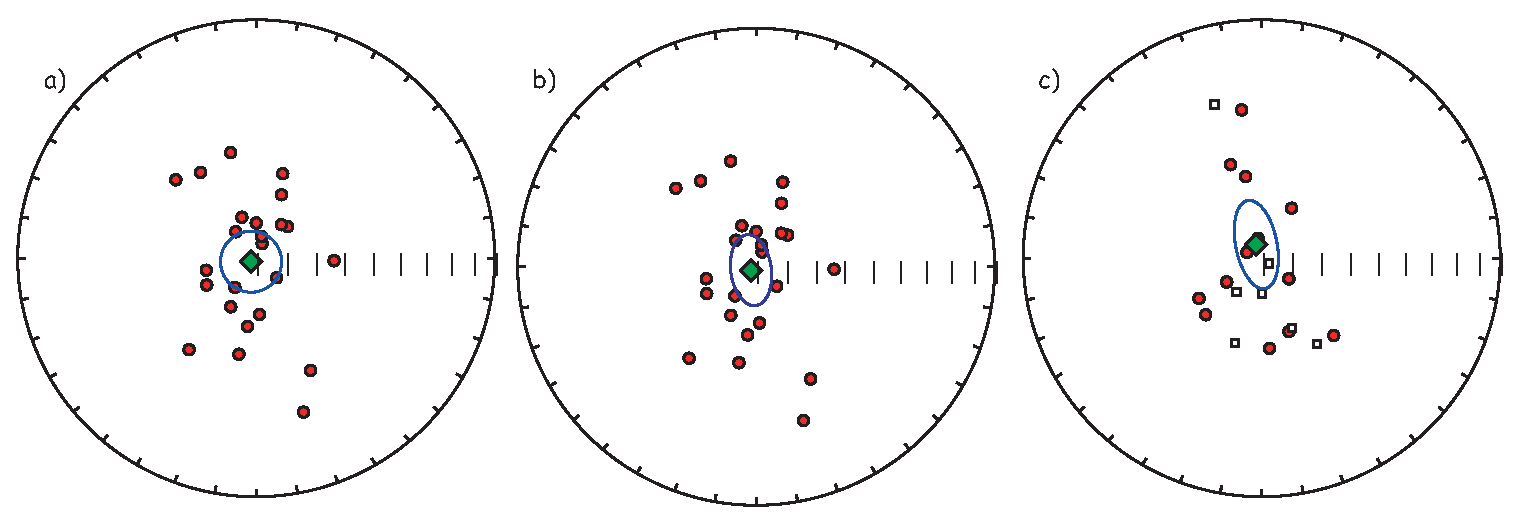
\includegraphics[width= 14 cm]{EPSfiles/confidence.eps}
\caption{ a) An example  of data obtained from a hypothetical equatorial sampling site plotted with the Fisher circle of confidence.   The data have been transposed such that the expected direction (0, 0) is at the center of the diagram and ``up'' is at the top.  b) Same data but with   the Kent 95\% confidence ellipse.  c) Data from a) with some directions transposed to the antipode; directions plotted with the Bingham 95\% confidence ellipse.  }
\label{fig:confidence}
\end{figure}
    

    
 \subsection{The Bingham distribution}
 
 The Kent distribution has the advantage that it can deal with elliptical data sets while the Fisher distribution cannot.  However, many paleomagnetic data sets are also bi-modal (reversals!) and the Kent and Fisher distributions can only deal with data sets with a single polarity.    It was precisely for the purpose of treating bimodal, elliptical data that the 
\index{distributions!Bingham}
 Bingham distribution was developed 
 \index{Bingham, C.}
 (Bingham, 1974).    \nocite{bingham74}   The Bingham distribution is given by:
 
 $$
 F = {1\over {4\pi d(k_1,k_2)} } \exp( k_1\cos^2 \phi+k_2\sin^2\phi)\sin^2 \alpha,
 $$
 \noindent where $\alpha$ and $\phi$ are as in the Kent distribution,  $k_1,k_2$ are concentration parameters ($k_1<k_2<0$) and $d(k_1,k_2)$ is a constant of normalization. Values for $k_1,k_2$ can be estimated by numerical integration and can be converted into 95\% confidence ellipses, the details of which are  given in Appendix~\ref{app:bing}.   In a nut shell, the $\V_1$ eigenvector   of the orientation matrix (associated with the largest eigenvalue,  see Appendix~\ref{app:eigen}) is the principal direction and the semi-axes of the 95\% confidence ellipse  are proportional to the intermediate and minimum eigenvalues.  The Bingham principal direction therefore is not necessarily  the same as the Fisher or Kent  mean.  If we take each vector end-point to be a mass, the Bingham principal direction is the axis about which the moment of inertia of the masses would be least.  The Fisher mean is somewhat different, in that it is the vector sum of unit vectors.  The Bingham  mean (principal direction) is less affected by outliers than the Fisher mean, lying closer to the center of mass of data points.   
 
 The principle drawback of the Bingham distribution is that because the orientation matrix uses the entire data set (normal and reverse) the two modes are assumed to be antipodal and to share the same distribution parameters.  The question of whether normal and reverse data sets are antipodal and have the same dispersion is in fact one we may wish to ask!    One could separate the two modes prior to calculation of the 
 \index{Bingham!confidence ellipse}
 Bingham ellipse, but then the rationale for using the Bingham distribution is lost.  Also, many published descriptions of the Bingham calculation (e.g.,
 \index{Onstott, T.}
 \index{Borradaile, G.J.}
Onstott et al. 1980, Borradaile,  2003)  \nocite{onstott80,borradaile03}  have errors in them.   The source code for calculating Bingham statistics in widely used  paleomagnetic data reduction programs  is generally not available, and it is unknown whether these programs contain bugs.   
 
 \subsection{The Bingham-LeGoff approximation}
 
 Estimating the parameters for the Bingham ellipse exactly is computationally taxing and all of the available ``canned'' programs use the look up table of 
 \index{Mardia, K.V.}
 \index{Zemroch, P.J.}
 Mardia and Zemroch (1977;  see Appendix~\ref{app:bing}).  \nocite{mardia77}
 \index{LeGoff, M.}
  LeGoff et al. (1992) \nocite{legoff92} suggested some approximations which may be valid for concentrated distributions.   They also introduced the concept of weighting results according to  some reliability criteria.   For the general case, however, it seems preferable to use the exact
  \index{Kent, J.T.} Kent (1982) \nocite{kent82}
  ellipses on uni-modal data sets.  These could of course be weighted if such weighting is desired.  
 
 
 \begin{figure}[htb]
%\epsfxsize 12cm
%\centering \epsffile{EPSfiles/love.eps}
\centering  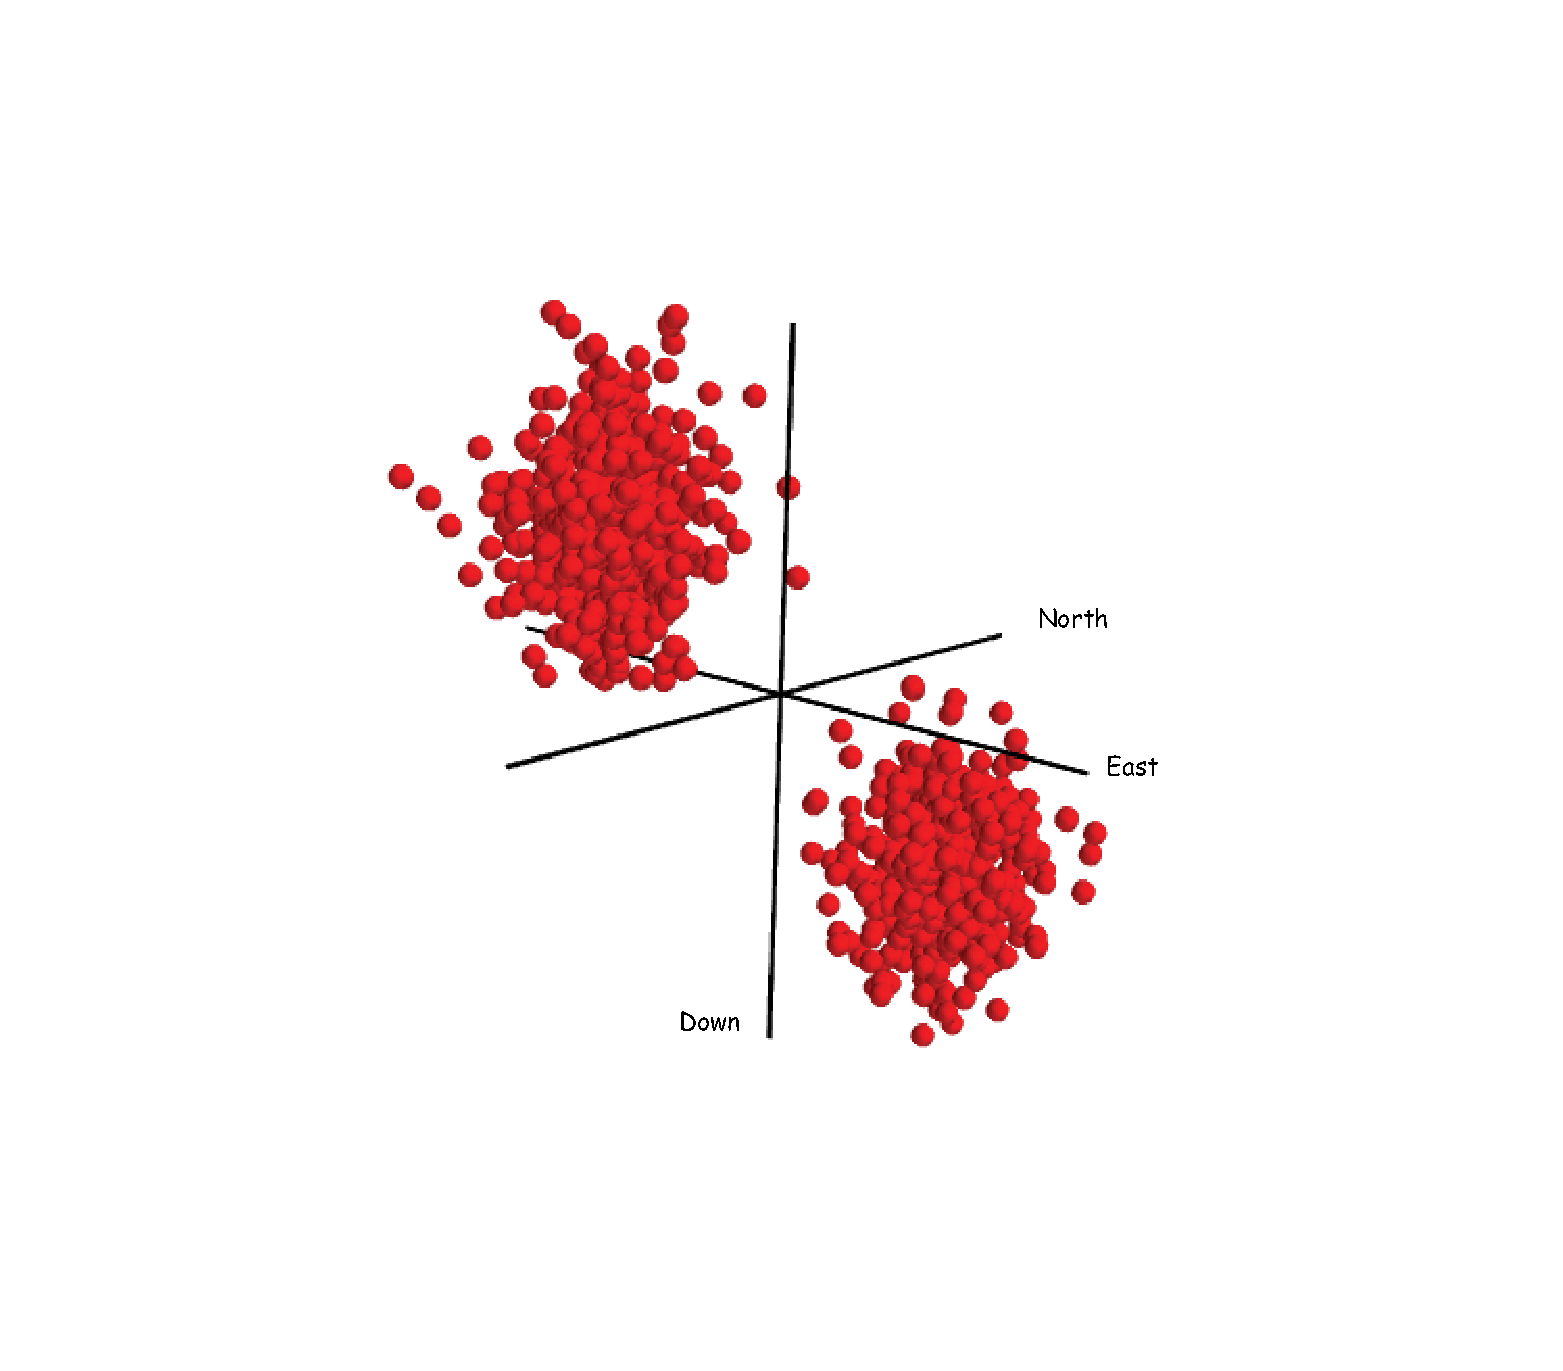
\includegraphics[width=12 cm]{EPSfiles/love.eps}
\caption{A bi-gaussian set of vectors suitable for treatment using the method of Love and Constable (2003).  }
\label{fig:love}
\end{figure}\nocite{love03}

\subsection{The Bi-Gaussian distribution}

\index{distributions!bi-gaussian}       
Until now we have continued the Fisher assumption of unit vectors.  As already mentioned,  neglect of the vector strength  can lead to bias.  
\index{Love, J.J.}
\index{Constable, C.G.}
 Love and Constable (2003) \nocite{love03}
began the hard work of incorporating intensity information into the parameter estimation problem.  Their method can handle bi-modal spherical Gaussian data such as those shown in Figure~\ref{fig:love}. Estimation of the Love parameters are beyond the scope of this book.   Moreover, many data sets are not spherically symmetric as already noted and the Love and Constable (2003) approach must be generalized to elliptical, more ``blade-like'' data sets than the ``cotton balls'' currently treatable.  


 \begin{figure}[htb]
%\epsfxsize 14cm
%\centering \epsffile{EPSfiles/hypeq.eps}
\centering  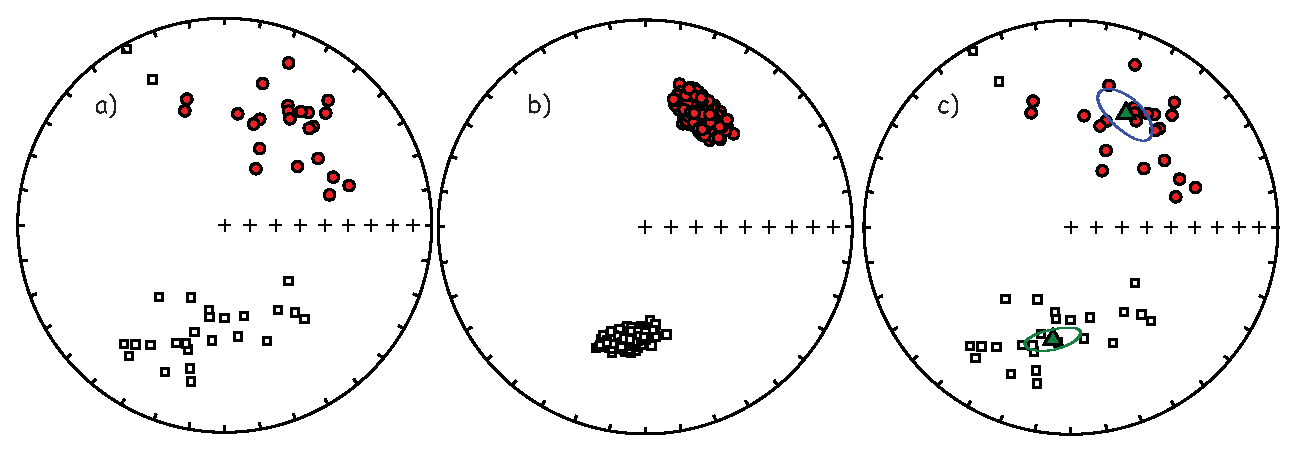
\includegraphics[width=14 cm]{EPSfiles/hypeq.eps}
\caption {a) Hypothetical non-Fisherian data set.  Normal and reversed polarity data that are not symmetrically distributed. Filled (open) circles plot on the lower (upper) hemisphere.  b) Equal area projection of 500 bootstrapped means for pseudo-samples drawn from the data shown in    a).    c) Same as a) but with the bootstrapped confidence ellipses shown. }
\label{fig:hypeq}
\end{figure}



\section{The simple (na\"ive) bootstrap}

As we have mentioned,  real data may  be pathological in several respects including  bi-modal and elliptically distributed data.   None of the methods we have described so far  have the  
\index{statistical tests!bootstrap!common mean direction}
test for common mean so critical to paleomagnetic studies nor can they provide confidence ellipses for  an off-center mean direction
  as  is likely to occur in records of the geomagnetic field (see Figure~\ref{fig:vgp-di}b).  Finally, data may be overprinted or contain the record of a paleomagnetic transition, resulting in ``streaked'' or non-antipodal distributions, conditions that make the conventional methods inappropriate.    In this section we will discuss alternative methods for estimating confidence bounds which are sufficiently flexible to accomodate all of these short comings, provided the data set is large enough.  

In Figure~\ref{fig:hypeq}a we show a not unusual ``not great'' paleomagnetic data set.  The data are   elliptical, bi-modal and one has the suspicion that the normal and reverse modes may be neither antipodal nor share the same concentration or ovalness parameters.  Clearly some non-parametric approach would be desirable.  
The  approach for   characterizing uncertainties for vectors we will take here is based on a technique known as the statistical 
{\it bootstrap}.  As we shall see, the bootstrap has the flexibility to allow us to treat awkward data sets like that shown in Figure~\ref{fig:hypeq}a.  

The principles of the bootstrap  are given in Appendix~\ref{app:bootstrap}.  In essence, the parameter of interest (say, the mean vector) is calculated from many resampled data sets, whose data points are selected at random from  the original data.   The bootstrapped estimates ``map out'' the likely distribution of the parameter, allowing estimation of confidence regions.   Before we extend the bootstrap from the scalar treatment in Appendix~\ref{app:bootstrap}  to vectors, it is important to point out that  with the bootstrap, it is assumed that the underlying distribution is
represented by the data, demanding that the data sets be rather
large.   Moreover, the bootstrap estimates are only asymptotically
valid, meaning that a large number of bootstrap calculations are required
for the confidence intervals to be valid.    It's a good thing we have fast computers with huge hard-drives.


 
There are a variety of ways we can use the bootstrap to estimate confidence regions for paleomagnetic data.  We will start with the most ``Fisher'' like approach of taking unit vectors of a single polarity.  Then we will accommodate dual polarity data sets and develop analogous tests to those so useful for Fisher distributions.  

To do a simple 
\index{bootstrap!directions}
\index{bootstrap!na\"ive}
bootstrap on a data set with only one polarity (say the normal data in Figure~\ref{fig:hypeq}a,  we first 
 randomly draw $N$ data points from the data shown in
Figure~\ref{fig:hypeq}a.  
Each set of $N$ data points is a {\it pseudo-sample}. Note that some data points will be drawn more than once while others will not be drawn at all in a particular pseudo-sample.  We then calculate a Fisher mean of the pseudo-sample (one little circle in Figure~\ref{fig:hypeq}b.  This resampling procedure can be repeated many times.  We show 500 such bootstrapped means in Figure~\ref{fig:hypeq}b.    
 
Now we can estimate the region of 95\% confidence for the
bootstrapped means.  A non-parametric approach would be to
draw a contour enclosing 95\% of the bootstrapped means.   In many applications,
paleomagnetists desire a more compact way of expressing
confidence regions (for example, to list them in a table)
and this necessitates some parametric assumptions
about the distribution of the means.   For this limited purpose,
approximate 95\% confidence regions can be estimated by noting the elliptical distribution of the bootstrapped means and by assuming that they are  
\index{Kent, J.T.}
\nocite{kent82}
Kent (1982) distributed.  Such bootstrap confidence ellipses are shown in Figure~\ref{fig:hypeq}c.  

 When paleomagnetic data are bimodal,  as in Figure~\ref{fig:hypeq}a, we can proceed in one of two ways.  We could just calculate the principal eigenvector of the orientation matrix ($\V_1$) as in Bingham statistics  of each bootstrapped pseudo-sample or we can separate the data into two modes and calculate Fisher means for each mode separately (as in Figure~\ref{fig:hypeq}b).    

 To  separate the data into normal and reverse subsets, we first calculate the principle direction of the whole dataset.   This will be more or less parallel to the Fisher mean of one of the modes.  Any direction more than 90$^{\circ}$ away from this could be placed in the second mode.      After separation, Fisher means of the bootstrapped pseudo-samples can be calculated for each mode separately.   Alternatively, if a
more robust estimate of the ``average'' direction is desired, one could calculate the 
principal eigenvector $\V_1$ of each mode, which is less sensitive to the presence of outliers.



\begin{figure}[htb]
%\epsfxsize 11cm
%\centering \epsffile{EPSfiles/twofiles.eps}
\centering  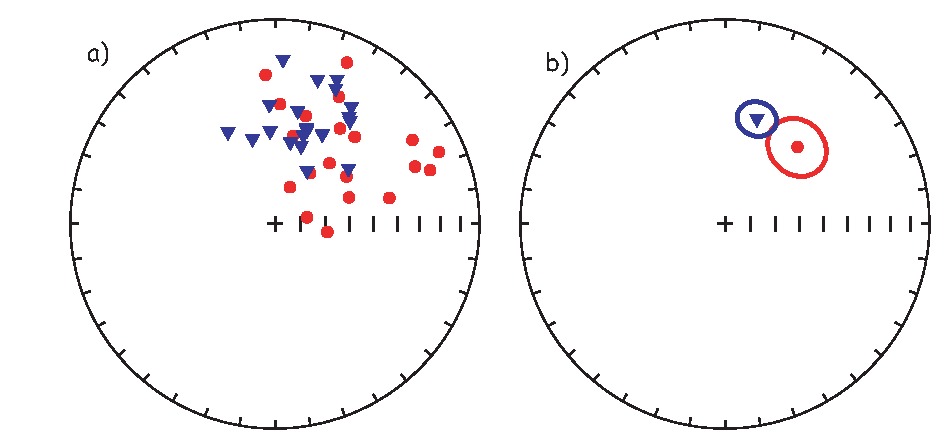
\includegraphics[width=11 cm]{EPSfiles/twofiles.eps}
\caption {Test for common mean with two directional data sets. 
a) Equal-area projections of   two
simulated Fisherian data sets  (triangles and circles) each with $\kappa$ of 20.  b) Means and $\alpha_{95}$s of  data sets shown in a).  }
\label{fig:twofiles}
\end{figure}


\section {The parametric bootstrap}


The bootstrap just described is a  ``simple'' or ``na\"ive'' bootstrap in that
no distribution is assumed for the data.  We did assume, however, that all the
uncertainty inherent in the data is reflected in the data distribution.
 If the data set is smaller than about $N=20$, this leads to
uncertainty ellipses that are too small  
\index{Tauxe, L.}
(Tauxe et al., 1991).  \nocite{tauxe91}
Many paleomagnetic data sets are smaller than this,  yet they
are demonstrably non-Fisherian.  Luckily, if we are able to assume some
parametric form for  data from e.g.,  a given site, we can use a superior
technique which is known as the 
\index{bootstrap!parametric}
{\it parametric bootstrap}.  As applied here, we assume
that each site with $N$ samples is Fisher distributed (in principle,
a testable assumption).
Then, after random selection of a particular site for inclusion in the 
pseudo-sample, we draw $N$ new directions from a Fisher distribution with the
same mean direction, $\kappa$ and $N$. From these simulated data sets, we calculate a 
substitute mean direction, and use that
in the pseudo-sample.  Otherwise, we follow the same procedure as
in the simple bootstrap.

For large data sets ($N>25$), the parametric and simple bootstraps yield
very similar confidence ellipses.   For smaller data sets, the parametric ellipses
are larger, and are probably more realistic.  


\begin{figure}[htb]
%\epsfxsize 14.5cm
%\centering \epsffile{EPSfiles/cdf.eps}
\centering  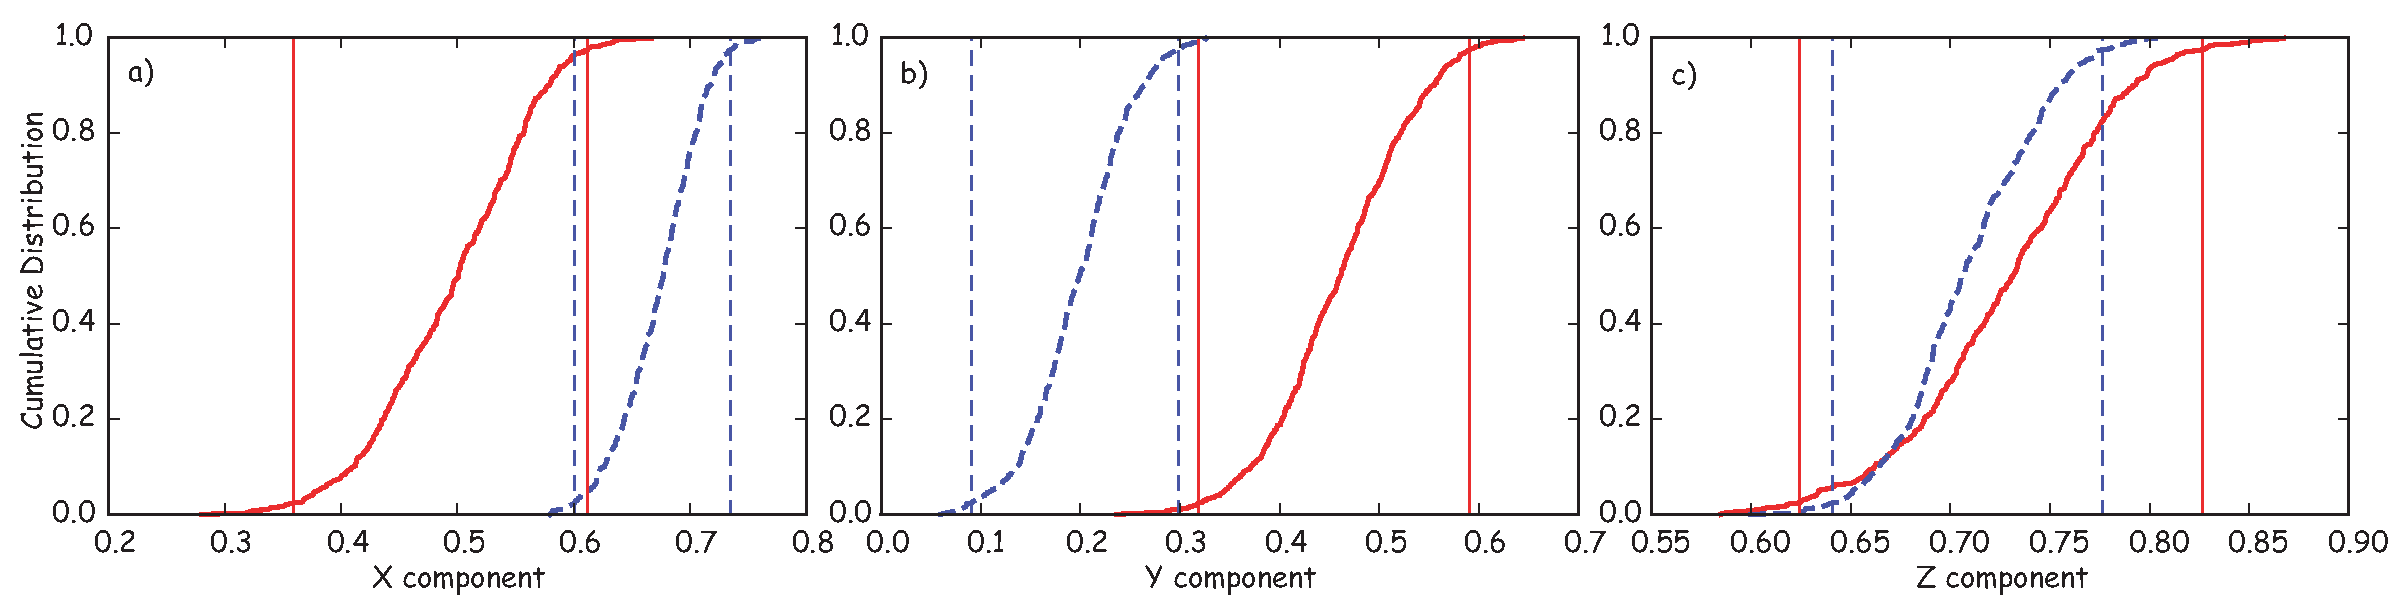
\includegraphics[width=14.5 cm]{EPSfiles/cdf.eps}
\caption{
Cumulative distributions of 
Cartesian  components  of the bootstrapped means from 500 pseudo-samples from data shown in Figure 12.5. a) $X$ components.  b) $ Y$, and c) $Z$.
Also shown are the bounds for each data set that include 95\% of the 
components.
The confidence intervals for the different data sets 
overlap for $X$ and $Z$ but not for $Y$.  
  }
  \label{fig:cdf}
  \end{figure}


\section{When are two data sets distinct?}
 

The test for a common mean addresses the question ``can the means of two data
sets be discriminated from one another?''  
Another way of putting it is,  ``If a set of bootstrap means is examined, 
are there two distinct groups or is there
just one?''  We explore these ideas by considering  the same Fisherian data sets
we used in Chapter 11 for the Watson's $V_w$ test.  
In Figure~\ref{fig:twofiles} we show  two data sets (triangles and circles), 
each drawn from distributions with a $\kappa$ of 20.
The mean direction of each lies outside the confidence region of the other and the  $V_w$ test of 
 \index{Watson, G.S.}
\index{statistical tests!Watson's $V_w$}
 Watson (Chapter 11) has a value of 11.7 with a critical value of 6.3; hence the data sets  fail the test for a common mean. 

In order to develop a bootstrap test analagous to the $V_w$ test for use on non-Fisherian data sets, we first convert a set of bootstrapped mean  directions 
to Cartesian coordinates. Cumulative distributions of the Cartesian coordinates of the
bootstrap means  are shown in Figure~\ref{fig:cdf}a-c along with the bounds containing 95\% of the means for each data set.    The two sets of directions are distinct in the $Y$ component, confirming that the two means can  be distinguished at the 95\% confidence level.


\section {Application to the ``reversals test''}

The so-called 
\index{statistical tests!bootstrap!reversals}
{\it reversals test} in paleomagnetism constitutes a test
for a common mean for two modes, one of which has been ``flipped'' to
its antipode.  We apply our bootstrap test for common mean to the data shown
in Figure~\ref{fig:hypeq}.  The cumulative distributions of the Cartesian coordinates
of the bootstrapped means are shown in Figure~\ref{fig:revtest}.  The confidence intervals
for the normal and reverse antipodes overlap, thereby  suggesting  that the two
means cannot be distinguished at the 95\% level of confidence.  
 Thus,  the data in Figure~\ref{fig:hypeq} pass the bootstrap reversals test.  


 \begin{figure}[h!tb]
%\epsfxsize 14cm
%\centering \epsffile{EPSfiles/revtest.eps}
\centering  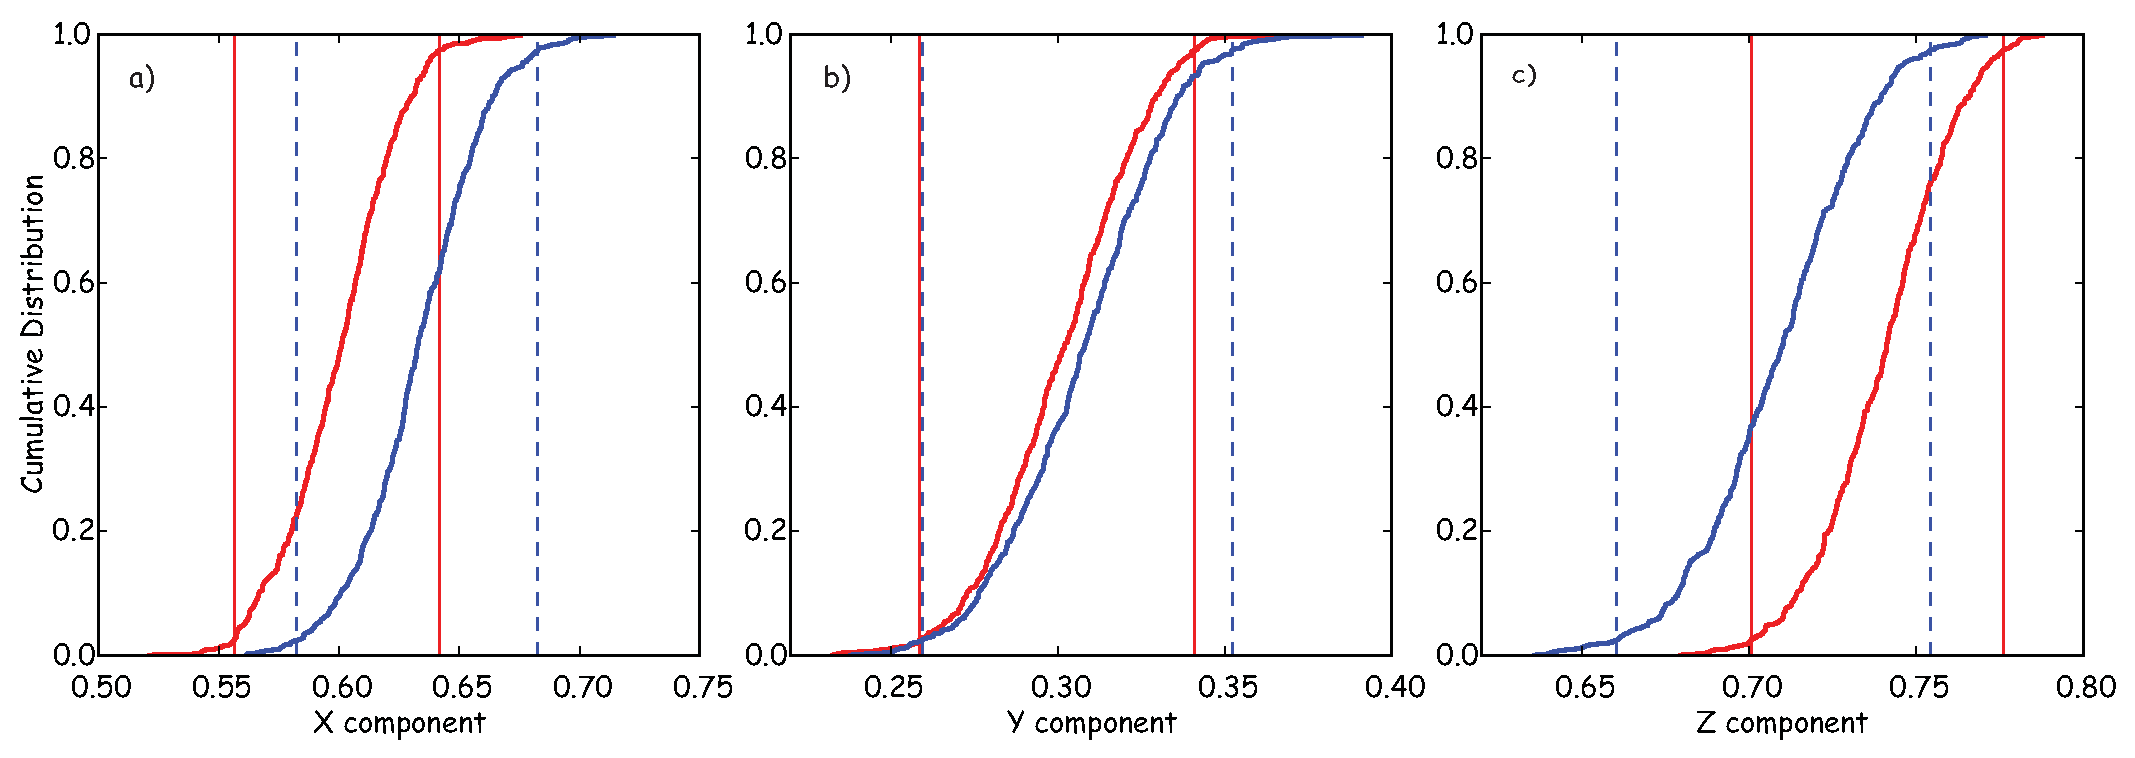
\includegraphics[width=14 cm]{EPSfiles/revtest.eps}
\caption{Cumulative distributions of Cartesian coordinates of  means of 
pseudo-samples drawn from the data shown in
Figure 12.4a. The reverse polarity mode has been 
flipped to its antipode.  The intervals containing 95\% of each
set of components are also drawn (vertical lines).
  Because the confidence bounds from the two  data sets overlap in all
three components, the means of the reverse and normal modes  cannot
be distinguished at the 95\% level of confidence; they pass the
bootstrap reversals test.}
\label{fig:revtest}
\end{figure}



\section {Application to the ``fold test''}

A final test is useful in paleomagnetism: the 
\index{paleomagnetic tests!fold!bootstrap}
 fold
test (Chapter 9).  
 If a rock has moved from its original
position, was  it magnetized in the original,  in the present  or in
some other position?  Moreover, is simple rotation about strike an
appropriate method to restore the beds to their original positions?
In the classic fold test envisioned  by 
\index{Graham, J.W.}
Graham (1949),   \nocite{graham49}  (see Chapters 9 and  11),
the
directions of magnetization of a deformed rock unit are assumed to be
most closely
parallel in the orientation in which the magnetization was acquired.
Therefore, if
a rock has retained an original magnetization through a subsequent
folding or
tilting event, the magnetic directions may cluster most tightly after
they have been rotated back to their original positions.  This of course is not necessarily true for elongate data such as those shown in Figure~\ref{fig:confidence}a for which we can imagine pathological cases that result in a more tightly clustered set of directions in a coordinate system other than the one the data were magnetized in.  Nonetheless, the clustering assumption is probably reasonable in most scenarios.  



The fold test appears at first glance
 to be simple, but it is not.
The primary problem is that paleomagnetic
vectors are never perfectly parallel.  The
scattered nature of the data means that a statistical test is
necessary to determine whether clustering is ``significantly'' better
in one orientation or another.


In Chapter 11 we suggested that variances could be compared using an F-test, so it was long the practice in paleomagnetism to compare estimated precisions  before and after tilt adjustment
\index{McElhinny, M.W.}
 (McElhinny, 1964). \nocite{mcelhinny64}
The ratio of the two estimates of $\kappa$ were 
 compared 
with those listed in statistical
\index{distributions!$F$}
 F-distribution tables. Ratios higher than  the 
$F$ value for a given $N$ were deemed to constitute a significant increase in
concentration after adjusting for tilt,  thus representing
 a positive fold test.  This
test can be done on the back of an envelope and  is still in frequent use.

\begin{figure}[htb]
%\epsfxsize 14cm 
%\centering \epsffile{EPSfiles/unfolding.eps}
\centering  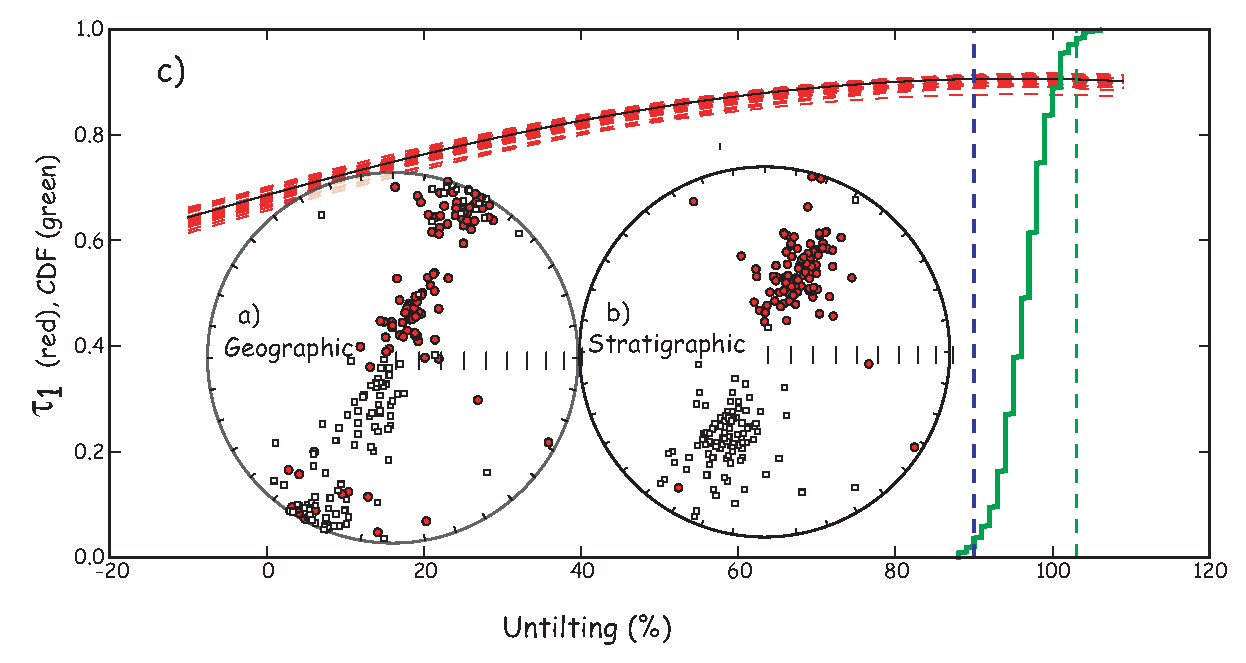
\includegraphics[width=14 cm]{EPSfiles/unfolding.eps}
\caption{
a) Equal area projection of a set of directions in geographic coordinates.
The data were drawn from the same distribution  of directions that gave rise to the VGPs shown in Figure 12.1a.  They have been rotated about strike on two simulated limbs of the fold, one to the northeast and one to the southwest, resulting in  a streaked (girdle) distribution.  The  original polarity of many
data points is ambiguous.  b) Data from a) after back tilting by  100\% of the original tilt.     Polarities
are more readily identifiable.  
c) Red dashed lines: trends of the largest eigenvalues ($\tau_1$s) of the orientation matrices
from representative pseudo-samples drawn from a) as they evolve during untilting.  The
directions are adjusted for tilt incrementally from -10\% to 110\%.  The
largest value of ($\tau_1$ occurs near 100\% in all of the pseudo-samples
sets. The cumulative distribution is of 500 maxima of $\tau_1$ and the bounds that enclose 95\% of them.     These data
``pass'' the bootstrap fold test.}
\label{fig:foldtest}
\end{figure}

Although its simplicity is a great strength, there are several problems with the
classical  fold test.
  First, the  geomagnetic field has two preferred states and is not perfectly dipolar.
Directions observed in paleomagnetic samples are therefore not only
scattered but are often of two polarities.
Second, the magnetic directions may be most tightly clustered somewhere other than in
``geographic'' or 100\% tilt adjusted coordinates (McCabe et al., 1983). \nocite{mccabe83}     Finally, structural
``corrections'' are not perfectly known.  Not only are the bedding
orientations themselves often difficult to measure
accurately, but detection of complications such as plunging folds, and
multiple phases of tilting requires
extensive field work.  It is nearly impossible to assess
rotation about the vertical axis on the basis of field relations alone,
as it results in no visible effect on the dip of the beds themselves.
Because of this uncertainty, we might reasonably ask whether if the data are actually
most tightly clustered at, say 90\% tilt adjusted (as opposed to 100\%), does this
constitute a ``failed'' fold test.
 
We consider first the problem of dual polarity.  We plot a hypothetical data 
set in geographic coordinates in Figure~\ref{fig:foldtest}a and in tilt adjusted coordinates in Figure~\ref{fig:foldtest}b.  The polarity is ambiguous but the classic fold test
requires calculation of $\kappa$ which can only be done with data of a single
polarity.  Obviously, fold tests that rely on $\kappa$ will not 
be straight forward with data such as these.

An alternative approach  is based on the orientation matrix 
\index{Tauxe, L.}
\index{Watson, G.S.}
(Tauxe and Watson, 1994).   \nocite{tauxe94} [Please read Appendix~\ref{app:eigen} if you have not yet done so.]
 In the
orientation matrix, polarity does not  play a role and the ``tightness'' of
grouping is reflected in the relative magnitudes of the eigenvalues ($\tau$).  
As the data become more tightly grouped, the variance along the principal
axis grows and those along the other axes shrink. Thus, examination of the
behavior of $\tau_1$ during unfolding would reveal the point at which
the tightest grouping is achieved, without knowledge of polarity.    



Suppose we find that the degree of unfolding required to
produce the maximum in $\tau_1$ is 98\%.  Is this a positive fold test
suggesting a pre-folding remanence or is the difference between 98\% and
100\% significant?  For this we call on the by now familiar bootstrap.  
Numerous pseudo-samples  can be drawn. We can then calculate the 
eigenparameters of the orientation matrix
for a range of  percent unfolding.  Some
examples of the behavior of $\tau_1$ during tilt adjustment of representative
pseudo-samples drawn from the data
in Figure~\ref{fig:foldtest}a are shown 
in Figure~\ref{fig:foldtest}c.  The green line in Figure~\ref{fig:foldtest}c is a cumulative distribution plot of maxima in
$\tau_1$ from 500 pseudo-samples.  These are sorted   and the 95\%
confidence interval for the degree of unfolding required to produce the
tightest grouping (the highest $\tau_1$)
 is  thus constrained to lie between 97 and 102\%.  



The data from Figure ~\ref{fig:foldtest}a are shown after 100\% tilt
adjustment
in Figure~\ref{fig:foldtest}b. The tilt adjusted
  data are not only better grouped, but now
the polarities of most samples can be readily determined.  An advantage 
of the eigenparameter
approach is the fact that the data do not need prior editing to
split them into normal and reversed polarity groups, which is  a particularly onerous task
for the data considered here.

For small data sets,  we could  employ a parametric bootstrap, whereby
pseudo-samples are generated by first randomly selecting a site for
inclusion, then by drawing a substitute direction from a Fisher distribution
having the same $D$, $I$, $N$, and $\kappa$. 

We can incorporate uncertainties in bedding into the bootstrap.  If we assume that the poles to the bedding planes are Fisher distributed, and we can assign some estimated $\kappa$ value to the distribution of poles based on repeat measurements (say, $\kappa \simeq $ 30), we can draw poles to the beds from Fisher distributions using the assigned mean direction and $\kappa$.  We would then use these simulated poles in the structural corrections on the pseudo-samples.  This procedure would propagate the uncertainties in structural corrections through the fold test, resulting in more realistic confidence bounds on the peak in concentration during unfolding.   

Finally, it is important to remember that peaks in concentration between 0 and 100\% unfolding can result from a variety of causes. \nocite{tauxe94}   Traditionally, intermediate peaks have been interpreted as resulting from remagnetization  of the rock units during folding (see, e.g., McCabe et al., 1983). \nocite{mccabe83}  Such behavior could also result from failure to account for plunging folds, or vertical axis rotation between blocks  (see Tauxe and Watson, 1994), so some caution should be exercised when interpreting fold test results.  

\vskip 12pt
\noindent SUPPLEMENTAL READINGS: Fisher,  et al. (1987), Chapters 2--5.  \nocite{fisher87}

\vskip 12pt

\section{Problems}

{\parindent 0pt  \parskip 8pt

{\bf Problem 1 }

 Change directories into Chapter\_12 (see the Problems in Chapter 5 for downloading instructions.)    This problem set will use the {\bf PmagPy} programs on the command line.  You can check the \href{http://earthref.org/PmagPy/cookbook/}{PmagPy website} for examples in how to use the {\bf PmagPy} programs. 
 
 a)
Look at {\it ps12-1a.di} with the program {\bf eqarea.py}.  Do the data look Fisher distributed to you?   
Now check whether they are using the program {\bf fishqq.py}.  Are they?   

b) Repeat this exercise for {\it ps12-1b.di}.  

c)  Now rotate the data in {\it ps12-1c.di}  to the mean direction.    Do this by first determining the mean  direction with {\bf gofish.py}.     Then use the program {\bf di\_rot.py} using the mean from {\bf gofish.py} as the new coordinate system.  Look at your output with {\bf eqarea.py} -- the center of the diagram will be the mean direction you used in {\bf di\_rot.py}.   Why are these data not Fisherian?  

{\bf Problem 2} 

a) The data in {\it ps12-2.dat} are $D, I$, dip direction and dip where the $D$ and $I$ are in geographic coordinates.   Use the program {\bf foldtest.py} to perform a fold test.  Were the data magnetized before or after folding?   

b) Repeat the fold test, but assign an angular uncertainty (CSD of the bedding pole distribution -- see Chapter 11) of 10$^{\circ}$.  Does this change your conclusion?  


{\bf Problem 3}

The data in {\it ps12-3.dat} are declination/inclination data from a paleomagnetic study. 

a)  First examine the data set  
with {\bf eqarea.py}.  

b) Separate the data into two files by polarity.  Calculate the Fisher means, and $\alpha_{95}$s with {\bf gofish.py}.  Check if the data are fisher distributed using {\bf fishqq.py}.   Calculate the Kent ellipses on the normal and reverse data sets using the program {\bf gokent.py}.  Calculate the Bingham ellipse on the whole data set using {\bf gobing.py}.  Now calculate the bootstrap ellipses using {\bf eqarea\_ell.py}.    Make plots of all the ellipses {\bf eqarea\_ell.py}.   Which method seems to represent the character of the data the best?

c) Now test whether or not  the two modes in the data are antipodal.    Use {\bf watsonsV.py} and {\bf revtest.py} to test whether the data pass a reversals test.    Do the data pass?  
Watson's $V_w$ test assumes a Fisher distribution, while {\bf revtest.py} uses a bootstrap and does not assume a Fisher distribution.   Which do you think should be used in this case?    Bingham statistics assumes that both polarities are the same, except for polarity, so you can not do a reversals test.   What are the advantages and disadvantages of the different methods for doing a reversals test? 

}
